\ifdefined\LONG
\begin{frame}{Linearizability}
An object has:
\begin{itemize}
\item state
\item a set of methods which operate on the object making the object move from one valid state to another
\end{itemize}
\begin{itemize}
\item A sequence of method invokations and responses is called a \emph{history}
\item Every method has a set of pre-conditions and post-conditions
\item Pre-conditions captures the state of an object before a method is invoked
\item Post-conditions captures the state after a method returns
\end{itemize}
\end{frame}

\begin{frame}{Linearizability}
\begin{itemize}
\item In a sequential specification of an object, each method is described in isolation
\item The interactions among methods are captured by the side-effects on the object state
\item So a sequential object needs a meaningful state only between method calls
\item New methods can be added without modifying the existing methods
\item proving correctness requires that the any history respects the sequential specification of the object
\end{itemize}
\end{frame}

\begin{frame}{Linearizability}
\begin{itemize}
\item For a concurrent object, multiple methods might be executing concurrently
\item Since method calls overlap, an object might never be between method calls
\item exponential possible interactions among method calls
\item Proving the correctness requires that some total ordering of any history respects the sequential specification of the object
\end{itemize}
\end{frame}

\begin{frame}{Linearizability}
Linearizability requires two properties:
\begin{itemize}
\item the object (or data structure) be sequentially consistent\footnote{\textit{\tiny the result of any execution is the same as if the operations of all the processors were executed in some sequential order, and the operations of each individual processor appear in this sequence in the order specified by its program}}
\item the total ordering which makes it sequentially consistent respect the \emph{real-time ordering} among the operations in the execution
\end{itemize}
\emph{respecting real-time ordering} - if an operation $op_1$ completed before another operation $op_2$, then $op_1$ must be ordered before $op_2$
\end{frame}

\begin{frame}{Linearizability}
\begin{itemize}
\item \emph{linearization point} - a distinct point between a method invokation and response where the method appears to have taken effect instantaneously
\item Order the method calls based on their linearization points
\item Resulting order should be in the sequential specification of the object.
\end{itemize}
\end{frame}
\fi

\begin{frame}{Linearizability}
\begin{center}
a correctness condition for concurrent objects
\end{center}
\pause
\begin{itemize}
\item methods - take time
\item methods - intervals with a start point (invocation) and an end point (response)
\item history - sequence of method invocations and responses
\end{itemize}
\end{frame}

\begin{frame}{Linearizability}
\begin{center}
Linearizability gives a total ordering of a history
\end{center}
\pause
\begin{itemize}
\item ordering of method calls w.r.t calls on the same thread should remain unchanged
\item overlapping method calls can be ordered based on the history
\item non-overlapping method calls across threads should preserve real-time ordering
\end{itemize}
\end{frame}

\begin{frame}{Linearizability - Examples}
\begin{figure}[htp]
		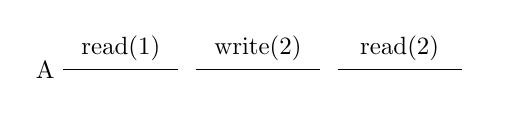
\begin{tikzpicture}[scale=0.9, transform shape] 
		\node (x1)  {A};
		\node (x2) [right of=x1,xshift=1cm]{};
		\draw (x1) -- node[above]{read(1)} (x2);
		\node(x3)[right of=x2,xshift=-1cm]{};
		\node(x4) [right of=x3,xshift=1cm]{};
		\draw (x3) -- node[above]{write(2)} (x4);
		
		\node(x5)[right of=x4,xshift=-1cm]{};
		\node(x6) [right of=x5,xshift=1cm]{};
		\draw (x5) -- node[above]{read(2)} (x6);
		\end{tikzpicture}
		\caption{A history of a sequential object}
\end{figure}
\end{frame}

\begin{frame}{Linearizability - Examples}
\begin{figure}[htp]
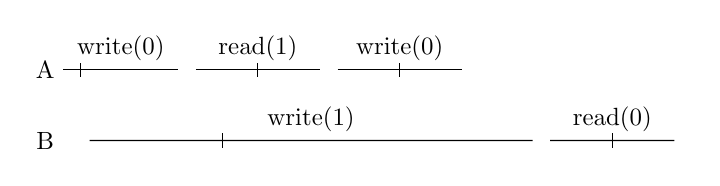
\begin{tikzpicture}[scale=0.9, transform shape] 
		\node (x1) {A};
		\node (x2) [right of=x1,xshift=1cm]{};
		\draw (x1) -- node[above]{write(0)} (x2);
		\draw (0.5,-0.1) -- (0.5,+0.1);
		
		\node(x3)[right of=x2,xshift=-1cm]{};
		\node(x4) [right of=x3,xshift=1cm]{};
		\draw (x3) -- node[above]{read(1)} (x4);
		\draw (3,-0.1) -- (3,+0.1);
		
		\node(x5)[right of=x4,xshift=-1cm]{};
		\node(x6) [right of=x5,xshift=1cm]{};
		\draw (x5) -- node[above]{write(0)} (x6);
		\draw (5,-0.1) -- (5,+0.1);
		
		\node(B)[below of=x1]{B};
		\node(x7)[below of=x1,xshift=0.5cm]{};
		\node(x8) [right of=x7,xshift=5.5cm]{};
		\draw (x7) -- node[above]{write(1)} (x8);
		\draw (2.5,-1.1) -- (2.5,-0.9);
		
		\node(x9)[right of=x8,xshift=-1cm]{};
		\node(x10) [right of=x9,xshift=1cm]{};
		\draw (x9) -- node[above]{read(0)} (x10);
		\draw (8,-1.1) -- (8,-0.9);
		
		\end{tikzpicture}
		\caption{A history of a concurrent object - linearizable}
\end{figure}
\end{frame}

\begin{frame}{Linearizability - Examples}
\begin{figure}[htp]
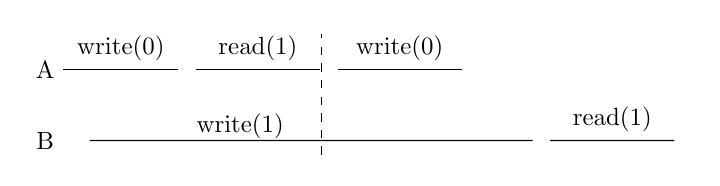
\begin{tikzpicture}[scale=0.9, transform shape] 
		\node (x1) {A};
		\node (x2) [right of=x1,xshift=1cm]{};
		\draw (x1) -- node[above]{write(0)} (x2);
		
		\node(x3)[right of=x2,xshift=-1cm]{};
		\node(x4) [right of=x3,xshift=1cm]{};
		\draw (x3) -- node[above]{read(1)} (x4);
		\draw[dashed] (3.9,-1.2) -- (3.9,+0.5);
		
		\node(x5)[right of=x4,xshift=-1cm]{};
		\node(x6) [right of=x5,xshift=1cm]{};
		\draw (x5) -- node[above]{write(0)} (x6);
		
		\node(B)[below of=x1]{B};
		\node(x7)[below of=x1,xshift=0.5cm]{};
		\node(x8) [right of=x7,xshift=5.5cm]{};
		\draw (x7) -- node [above, xshift=-1cm,yshift=-0.1cm] {write(1)} (x8);
		
		\node(x9)[right of=x8,xshift=-1cm]{};
		\node(x10) [right of=x9,xshift=1cm]{};
		\draw (x9) -- node[above]{read(1)} (x10);
		
		\end{tikzpicture}
		\caption{A history of a concurrent object - not linearizable}
\end{figure}
\end{frame}